\documentclass[10pt,a4paper]{article}
\usepackage{tikz} % for drawing figures
\usepackage{amsmath} % for equations
\usepackage{url} % for URLs
\usepackage{graphicx}
\usepackage{multicol}
\usepackage{varwidth}
\usepackage{blindtext}


\usepackage{linguex} % ** special include in directory: for doing handy example labeling and bracketing
\renewcommand{\firstrefdash}{} % used for linguex package not to put hyphens in example refs (1a instead of 1-a)
\usepackage{cogsci}
\usepackage{pslatex}
\usepackage{apacite}
\usepackage{placeins}

\newcommand{\sem}[1]{\mbox{$[\![$#1$]\!]$}}
\newcommand{\lam}{$\lambda$}
\newcommand{\gcs}[1]{\textcolor{blue}{[gcs: #1]}} 


% Possible title: Higher order pragmatic reasoning in reference games

\title{On the Purpose of Ambiguous Utterances}
\author{\large \textbf{our names}\\
our emails\\
our affiliations}


\begin{document}
\maketitle

\begin{abstract}
Viewed from a Gricean tradition, ambiguity in language is something to be avoided. 
However, ambiguity seems ubiquitous during conversations. 
We propose that sometimes speakers choose ambiguous utterances because they are interested in the opinions, preferences, and beliefs of others. 
We model this hypothesis by means of the rational speech act model (RSA), adding (i) a mechanism that infers listener’s priors when analyzing their responses to (ambiguous) utterances and (ii) the ability to choose utterances strategically for maximizing information gain.
Using an enhanced version of the original object choice experiment (Frank \& Goodman, 2012), our model fits participants’ data yielding variation explanations of more than $R^2>90\%$.
This shows that when monitoring the response of a conversation partner to an ambiguous utterance, we can learn something about the partner's preferences.
Moreover, speakers can choose utterances that are expected to yield most information about the listener's interpretation prior.
\textbf{Keywords:} 
ambiguity, pragmatics, information gain, predictive priors, Rational Speech Act model
\end{abstract}





\section{Introduction}
Traditionally, linguists have treated ambiguity as a bug in the communication system, something to be avoided or explained away \cite{grice1975,chomsky2002minimalism}.
More recent research has begun to take notice of the efficiency ambiguity affords to us: by relying on context to fill in missing information, we can reuse lightweight bits of language rather than fully specifying the intended message \cite{levinson2000,piantadosietal2012,wasow2015}. 
In this view, ambiguity serves as a feature---not a bug---of an efficient communication system.
This reasoning accords with years of psycholinguistic research documenting that speakers readily produce ambiguous utterances (see \citeNP{ferreira2008}, for an overview). 


Along related lines, \citeA{wasow2015} reviews a large body of evidence and concludes that ambiguity is rarely avoided, even in situations where it would be communicatively appropriate.
While this observation contradicts the Gricean maxim to avoid ambiguity (\citeNP{grice1975}).
Grice, in fact, only considered one case of strategic ambiguity, in which case it is the intention of the writer or speaker to in fact communicate both alternative interpretations that the ambiguous utterance affords. 
Thus, in such cases, the recognition of the ambiguity is the communicative purpose. \citeauthor{wasow2015}, on the other hand, reviews cases where ambiguity production seemingly neither serves any communicative purpose, nor triggers direct implicature. 


The current work identifies an additional benefit in using ambiguous language: the \emph{extra} information we gain from observing how our listeners resolve ambiguity.
We propose that language users learn about each other's private knowledge by observing how they resolve ambiguity. If language does not do the job of specifying the information necessary for full interpretation, then listeners are left to draw on their opinions, beliefs, and preferences to fill in the gaps; by observing how listeners fill those gaps, speakers learn about the opinions, beliefs, and preferences of the listeners.
In a dynamic, natural conversation then, speaker and listener take turns choosing ambiguous statements in order to leave room for the other to fill is, thus revealing mutual opinions, beliefs, and preferences to each other. 


By way of illustration, take, for example, the scenario in Fig.~\ref{FG-ref-game}. Suppose a speaker produces the single-word utterance ``blue'' in an attempt to signal one of the objects to a listener. The utterance is ambiguous; the listener can choose either the blue square or the blue circle. Suppose further that, upon hearing ``blue,'' the listener selects the blue circle. In observing this choice, the speaker learns something about the private thoughts of the listener: what made her select the blue circle instead of the blue square? Perhaps the circle is more salient to the listener, or the listener has a preference for circles, or the listener may believe that the speaker has a preference for circles, there may even be a mutual agreement that circles are to be preferred when possible. Importantly, by observing how the listener resolves the ambiguity in reference, the speaker can learn something about the private thoughts of the listener. 

\begin{figure}
	\centering
	\includegraphics[width=2in]{images/rsascene.eps}
	\caption{A simple reference game scenario from \citeA{frankgoodman2012}. In the game, speakers choose a single-word utterance to signal one of the objects to a listener. In this scenario, the speaker chooses between the utterances ``blue,'' ``green,'' ``square,'' and ``circle.''}\label{FG-ref-game}
\end{figure}

However, accessing this added information requires the speaker to reason pragmatically about the pragmatic reasoning of the listener---a higher-order pragmatic reasoning, as it were. In order select a referent, the listener must interpret the utterance. We follow \citeA{frankgoodman2012} in treating this interpretation process as active pragmatic, probabilistic reasoning: the listener interprets an utterance by reasoning about the process that generated it, namely the speaker, who selects an utterance by reasoning about how a listener would interpret it. \citeauthor{frankgoodman2012} model this recursive social reasoning between speakers and listeners, marking the launsch of the Rational Speech Act (RSA) modeling framework.

The current paper builds on the foundational, vanilla RSA model of reference games by introducing uncertainty about the prior beliefs of the listener and modeling a speaker who reasons about these beliefs on the basis of and in anticipation of the observed referent choice. 
We begin by walking through our modeling assumptions. 
We then present our model in full detail and test the behavioral predictions of our model against human data in a series of web-based experiments.
We conclude with a discussion of the significance of our findings for understanding ambiguity in natural language and relate the findings to current theories of predictive coding and active inference.


\section{Model}

We begin with the vanilla RSA model of \citeA{frankgoodman2012}. The recursive social reasoning inherent to the RSA modeling framework gets cashed out as various layers of inference. At the base, there is a hypothetical, na\"ive literal listener $L_0$ who hears an utterance $u$ and infers the state of the world $s$ that utterance is meant to describe, that is, the object that may be referred to by the utterance. $L_0$ performs this inference by conditioning on the literal semantics of $u$, \sem{$u$}. $L_0$ thus returns a uniform distribution over those states $s$ that can be truthfully described by $u$:
$$P_{L_{0}}(s|u) \propto \sem{$u$}(s).$$
One layer up, the speaker $S_1$ observes some state $s$ and chooses an utterance $u$ to communicate that state to $L_0$. $S_1$ chooses utterances on the basis of their utility for signaling $s$ to $L_0$, $U_{S_1}(u;s)$. The speaker's utility maximizes the probability that $L_0$ would arrive at the correct $s$ on the basis of $u$, $P_{L_{0}}(s|u)$, while minimizing the cost of $u$ itself, $C(u)$:
$$U_{S_{1}}(u;s) = \textrm{log}(P_{L_{0}}(s|u)) - C(u).$$
$S_1$ chooses utterances in proportion to their utility:
$$P_{S_{1}} (u|s) \propto   \textrm{exp}(\alpha \cdot U_{S_{1}} (u;s)).$$
At the top layer of inference, the \emph{pragmatic} listener $L_1$ infers $s$ on the basis of some observed $u$. The result is a distribution over likely states $s$; however, unlike $L_0$, $L_1$ updates beliefs about the world by reasoning about the process that \emph{generated} $u$, namely $S_1$. In other words, $L_1$ reasons about the $s$ that would have been most likely to lead $S_1$ to choose the $u$ that was observed:
$$P_{L_{1}}(s|u) \propto P_{S_{1}}(u|s) \cdot P(s).$$

\citeA{frankgoodman2012} tested the predictions of their model against behavioral data from reference games as in Figure \ref{FG-ref-game}. To model production behavior---which utterance should be chosen to communicate a given object---the authors generate predictions from $S_1$. To model interpretation behavior---which object is the speaker trying to communicate on the basis of their utterance---the authors generate predictions from $L_1$. Finding extremely high correlations between model predictions and behavioral data in both cases, \citeauthor{frankgoodman2012} have strong support for their model of pragmatic reasoning in reference games (see also \citeNP{qingfranke2015}, for a fuller exploration of the modeling choices).

Our model builds on the vanilla version of RSA above by allowing for uncertainty around the listener's state prior, $P(s)$. We have in mind a scenario where a listener might have a preference for a certain object feature (e.g., blue things, squares, circles, etc.), and these preference will influence their object choice. With this in mind, the speaker produces an utterance $u$, observes the listener's referent choice $s$, and, on the basis of that choice, infers the preferences $f$ the listener might have had when making it.
We use the same $L_0$ and $S_1$ from the vanilla model. However, we now parameterize $L_1$'s state prior so that it operates with respect to a given feature preference $P(s|f)$:
$$P_{L_{1}}(s|u,f) \propto P_{S_{1}}(u|s) \cdot P(s|f).$$
We then model a pragmatic speaker $S_2$ who updates beliefs about $L_1$'s preferences, $P(f)$. To do so, $S_2$ produces $u$, then observes $L_1$'s choice of $s$, and finally reasons about the likely feature preference $f$ that $L_1$ used to make that choice:
$$P_{S_{2}}(f|u,s) \propto P_{L_{1}}(s|u,f) \cdot P(f).$$
Moreover, we model the reasoning process by which a speaker selects the best utterance to learn about the preferences of the listener.
Starting with no knowledge of the listener's preferences, $S_2$ can be assumed to expect a uniform (i.e., flat) feature preference prior $P(f)$. The more the speaker's posterior beliefs about the preferences, $P_{S_{2}}(f|u,s)$, deviate from the uniform prior, the more the speaker will have learned about the listener's preferences. 
We can thus model this reasoning in the light of expected information gain, which can be equated with the attempt to maximize the KL divergence between speaker's prior and the expected posterior of the listener's feature preferences $f$, integrating over all hypothetically possible state observations $s$:
$$P_{b}(u) \propto \sum_{s:\  [\![u]\!](s)}\lambda \cdot \textrm{KL}(P(f),P_{S_{2}}(f|u,s))-C(u).$$

We now have two sets of predictions from our model to check: first, the pragmatic speaker's inference about the listener's feature preferences on the basis of their object choice; and second, the pragmatic speaker's strategic utterance selection in the light of the anticipated information gain about the listener's preferences considering their possible object choices $s$. Below, we present two experiments that test these predictions against human behavior.


\section{Expt.~1: Inferring preferences}

Our first task is to check the predictions of our $S_2$ layer: having observed that a listener selects some object $s$ in response to an utterance $u$, what are the most likely preferences the listener had when making their choice? 

\subsection{Participants}

We recruited 90 participants with US IP addresses through Amazon.com's Mechanical Turk crowdsourcing service. Participants were compensated for their participation. On the basis of a post-test demographics questionnaire, we identified 82 participants as native speakers of English; their data were included in the analyses reported below.

\subsection{Design and methods}

We presented participants with a series of reference game scenarios modeled after Figure \ref{FG-ref-game} from \citeA{frankgoodman2012}. Each scenario featured two people and three objects. One of the people served as the speaker, and the other served as the listener. The speaker asks the listener to choose one of the objects, but in doing so she is allowed to mention only one of the features of the target object. Participants were told that the listener might have a preference for certain object features, and participants were tasked with inferring those preferences after observing the speaker's utterance and listener's object choice.

We followed \citeA{frankgoodman2012} in our stimuli creation. Objects were allowed to vary along three dimensions: color (blue, red, green), shape (cloud, circle, or square), and pattern (solid, striped, polka-dotted). The listener's choice was chosen at random from the subset of the three objects that contained the uttered feature, and the speaker's utterance was chosen at random from the properties of the targeted object. By varying the object properties, the targeted object, and the utterance, we generated a total of 2400 scenarios. Speaker and listener names were chosen randomly in each trial. Participants saw the speaker's utterance in bold (e.g., ``green'' in Figure \ref{exp1-trial}) and the listener's choice appeared with a dotted orange outline (e.g., the leftmost object in Figure \ref{exp1-trial}). Based on the observed choice, participants were instructed to adjust a series of six sliders to indicate how likely it is that the listener had a preference for a given feature. The sliders specified the six feature values of the two feature dimension that were not mentioned in the speaker's utterance (e.g., pattern and shape in Figure \ref{exp1-trial}). Participants completed a series of $15$ trials. Objects and utterances were chosen as detailed above, with the constraint that 10 trials were potentially informative with respect to listener preferences and 5 trials were uninformative with respect to listener preferences (e.g., observing that the listener chose one of three identical objects). 

\begin{figure*}[ht!]
	\centering
	\includegraphics[width=4.5in]{images/exp1-trial.eps}
	\caption{A sample trial from \emph{Experiment 1: Inferring preferences}.}\label{exp1-trial}
\end{figure*}

\subsection{Results}

\begin{figure}[ht]
	\centering
	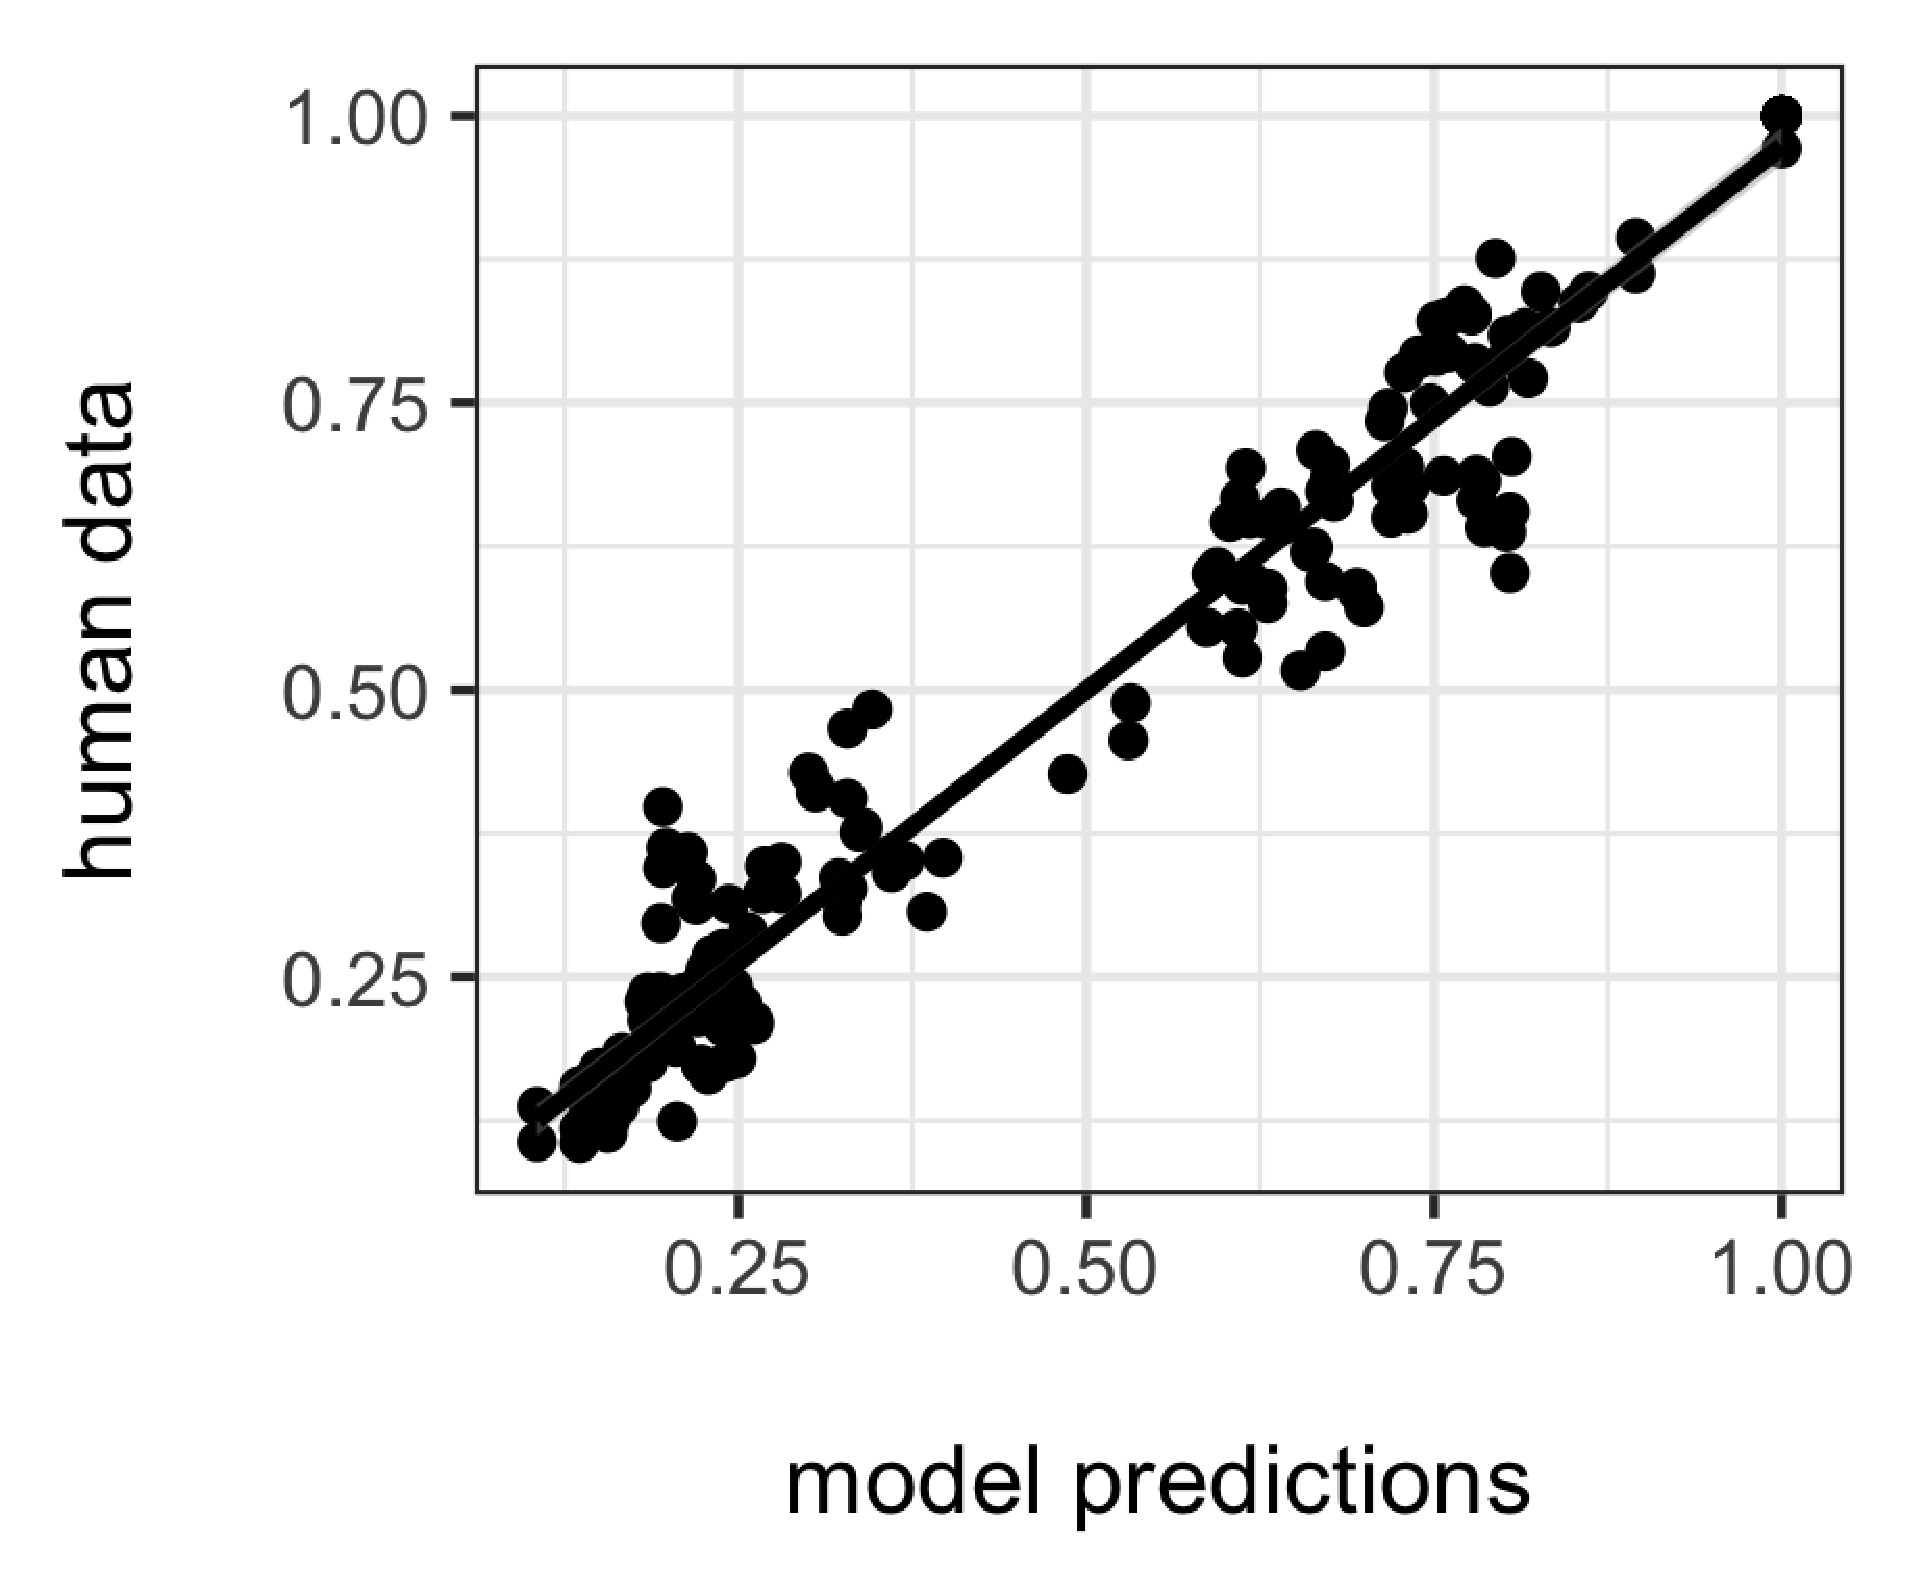
\includegraphics[width=3in]{images/X4-scatter-CogSci.eps}
	\caption{Experiment 1 results; $r^{2}=0.96$, 95\% CI [0.94, 0.97].}\label{exp1-results}
\end{figure}



% I used the code length(levels(as.factor(uniqueCCode))) to calculate the number of conditions

%Since not all of the stimuli allowed for inference of preferences in the same way, we introduced a new categorization of stimuli. Our base model would then predict the same preferences for the same category of stimuli. The categorization takes into account the distribution of features, the chosen object and which feature was uttered. Each category consists of 3 tuples of 2 digits. Each tuple refers to one feature, where the first tuple always refers to the uttered feature. The first digit in each tuple would then denote how many objects share the value of the picked object for the corresponding feature. In figure \ref{FG-ref-game}, if the utterance was blue and the blue square was picked, the first tuple would reference color and its first digit would be a "2". Note that this does not determine which other object shares the feature value, i.e. "blue". To compensate, the second digit of the tuple denotes which other object shares this value. This depends on the order of the objects -- we stipulated that the picked object would be the first. The further order would be determined by which other object shares this specific value, i.e. the "blue circle" in figure \ref{FG-ref-game} would be the first of the "other objects" and the "green square" the second. The picked object is at position zero in this sense. Thus the first tuple for figure \ref{FG-ref-game} would be (2,1). For the other tuples, the first digits would be "2" for shape and "3" for texture. To streamline the category code we stipulated that we would order the features in descending order of their first digit, so that we would have texture's "3" next in figure \ref{FG-ref-game}. If a tuple starts with "3" or "1", the second digit would simply denote whether the other objects have different values for that feature or the same. Thus we would have (3,2) for texture, with the second digit signaling that the non-picked objects share their texture. The tuple for shape would finally be (2,2), because the value "square" is shared with the second other object (see above). Thus for figure \ref{FG-ref-game} we would end up with [(2,1),(3,2),(2,2)].

The $S_2$ layer of our RSA model returns a posterior distribution over inferred feature preferences $f$ after observing a listener selecting an object in response to an utterance. 
Model predictions depend on two parameters.
The first is the soft-max scaling parameter $\alpha$ in the $S_1$ layer of the model, where the default value is typically set to $\alpha=1$. 
This parameter controls how likely $S_1$ is to maximize utility when choosing utterances. The second parameter scales the strength of individual feature preferences $f_i$. 
The softness parameter $\gamma$ determines how strong a preference is if a certain feature value is indeed preferred.
This parameter controls the shape of each of the possible feature preferences $f_i$ that $S_2$ considers. 
Preference softness increases with $\gamma$: 
a value of $\gamma=0$ specifies a hard preference, that is, if possible the listener will always choose the object that contains the preferred feature value. 
We assume $\gamma=0$ as the default model value. 
On the other hand, $\gamma \rightarrow \infty$ specifies a uniform feature value preference, that is, no actual preference.
As a result, a large value of $\gamma$ approximates a uniform prior default model such that the RSA models can be viewed as being nested within the default model.
% Note: I removed $\beta$ because it complicates things enormously and proved to be not really relevant.
%Finally, we allow for the possibility of noise in our human data introduced by participants not following instructions. The parameter $\beta$ \gcs{description of what $\beta$ does precisely}. As $\beta$ increases, speakers disregard instructions \gcs{summary of the effect}; at zero, speakers fully obey instructions. \gcs{summary of effect}.
%the For example, if a $S_2$ observes that following an utterance $blue$ and three objects all three of which are blue, but all differ in shape, the speaker chooses a square, the speaker might conclude that the $L_1$  has a preference for squares. However, the exact value on the slider the $S_2$ picks depends on the $\gamma$ parameter: if it is close to $0$, the speaker will mark that the $L_1$ had a perefernce for squares close to $1$. As the parameter value increases, the softness of preference will increase as well, drawing the preference value towards uniform (uninformative).
%he model contains three parameters: the informativity paramter $\alpha$ (how informative speakers choose to be), the obey-instructions parameter $\beta$, and the softness of preferences parameter $\gamma$. The latter 

% \gcs{We need to say something about how we fit individual participant data. How exactly where the parameter values fit? What were candidate values?}

We optimized $\gamma$, and $\alpha$ and $\gamma$ in the light of the KL divergence between the individual participants' slider value choices, and the according model predictions:
$$KL = \sum_{i=1}^{n}\textrm P(f'_i|u,s) (\textrm {log} (P(f'_i|u,s) - \textrm {log} (P(f_i|u,s)),$$
where $P(f_i|u,s)$ specifies the participant's normalized slider value settings, that is, feature preference posterior estimates, given an object scene with its particular utterance $u$, and object choice $s$, while $P(f_i|u,s)$ denotes the respective model prediction value.
Since not conclusions can be made about feature values that are not present in the scene, we ignored those respective feature preference estimates. 


By minimizing KL divergence between the empirical and model-predicted preferences for each participants, we maximize the model fit to the individual participants' data.
When compared to the uniform distribution based model, optimizing gamma yielded a much lower KL divergence value: while the uniform base model yields an average KL divergence of $9.848$ (median=$7.028$), our extended RSA model with individually optimized parameters $\gamma$, yielded an average KL divergence of $2.058$ (median=$1.524$). 
When optimizing $\alpha$ and $\gamma$ a yet smaller average KL divergence of $1.451$ (median=$0.952$) is reached.
In the light of the $G^2$ statistics and under the assumption that we calculated $2$ KL divergences in all $15$ trials per participant, the KL values should be multiplied by $2*15*2=60$ to yield a $G^2$ estimate, although, one may want to consider the two KL divergences in each trial as closely related, such that $2*15=30$ may be considered as a more passive multiplier.
With this factor, we get a difference of $233.7$ between the uniform base model and the one parameter extended RSA model, while the addition of $\alpha$ improves $G^2$ further by a value of $18.21$. Both of these are far above the cutoff value of $6.63$ for $p=.01$ assuming a Chi-square distribution \cite{Lewandowsky:2011}. 
Thus, the extended model exceeds the uniform base model with very high likelihood. 
However, seeing the much smaller improvement due to the optimization of $\alpha$ we analyze correlations with respect to the one-parameter, i.e., $\gamma$-optimized, model further. 
When considering the distribution of optimized parameters, we can identify three participants, which cause the optimization process to yield $\gamma$ values above $100$, indicating lazy participants who simply leave the slider values in the center. 
Another 15 yielded a $\gamma$ value above $1$, which is still considering preferences only to a small extent. The rest (i.e. 64 participants) yields values below $1$, indicating a strong consideration of preference inferences in line with the model. 
 

As traditionally is the case, though, RSA model predictions are compared to the human data in the light of the distinguishable interpretation cases. 
To do so, we identified all distinguishable cases in the light of the ambiguity of the chosen utterance and the possible object choices, essentially binning the data of all scenes with their utterances, for which the extended RSA model yields equal preference estimate posteriors. 
In the experiment with three objects that depict three feature values each out of three features with three feature-respective feature value options, there are $48$ scene types.
We binned those scene types 
For all bins, the actual feature values and objects in a scene were reordered according to the specific preference inference case. 
Thus, after reordering, the results of the individual slider values for individual scenes in each bin could be averaged for both, the participant's data and the model predictions. 


We plot predictions from the $\gamma$-optimized model in Figure \ref{exp1-results}.
A strong positive correlation between the human judgments and model predictions ($r^2 = 0.96, p < 0.001$) can be observed. Thus, we find strong empirical support for our extended RSA model of preference inference: speakers are indeed able to use listener behavior to arrive at information about their preferences. The question now turns to whether speakers are aware of the relative utility of different utterances when it comes to this reasoning. In other words, are speakers aware that ambiguous language is potentially more informative?



%\FloatBarrier 
% tried to keep figures in relevant sections but it doesn't look too good yet. Maybe when we have final text it will work out

\section{Expt.~2: Choosing utterances}

Our next task is to check the predictions of our strategic utterance selection model: given a set of potential referents, which utterance would be most informative with respect to the listener's preferences?

\subsection{Participants}

We recruited 90 participants with US IP addresses through Amazon.com's Mechanical Turk crowdsourcing service; participants in Experiment 1 were not eligible to participate in Experiment 2. Participants were compensated for their participation. On the basis of a post-test demographics questionnaire, as it happened, we identified again exactly 82 participants as native speakers of English; their data were included in the analyses reported below.

\begin{figure*}[ht]
	\centering
	\includegraphics[width=4.5in]{images/exp2-trial.eps}
	\caption{A sample trial from \emph{Experiment 2: Choosing utterances}.}\label{exp2-trial}
\end{figure*}


\subsection{Design and methods}

Participants encountered a reference game scenario similar to Experiment 1 in which a speaker signals an object to a listener who might have a preference for certain types of objects. However, rather than observing the utterance and referent choice, participants were now tasked with helping the speaker choose an utterance that was ``most likely to reveal the listener's color, shape, or pattern preferences.''

We used the same sets of objects from Experiment 1, which could vary along three dimensions. Each trial featured a set of three objects, as in Figure \ref{exp2-trial}. After observing the objects, participants adjusted sliders to indicate which single-feature utterance the speaker should choose. Potential utterances corresponded to the features of the objects present; depending on the number of unique features, participants adjusted between three and nine sliders, which specified the present feature values. Participants completed a series of 15 trials. As with Experiment 1, objects were chosen at random, with the constraint that 10 trials were potentially informative with respect to listener preferences (as in Figure \ref{exp2-trial}) and 5 trials were uninformative with respect to listener preferences (e.g., observing a set of three identical objects). 

\subsection{Results}

\begin{figure}[ht]
	\centering
	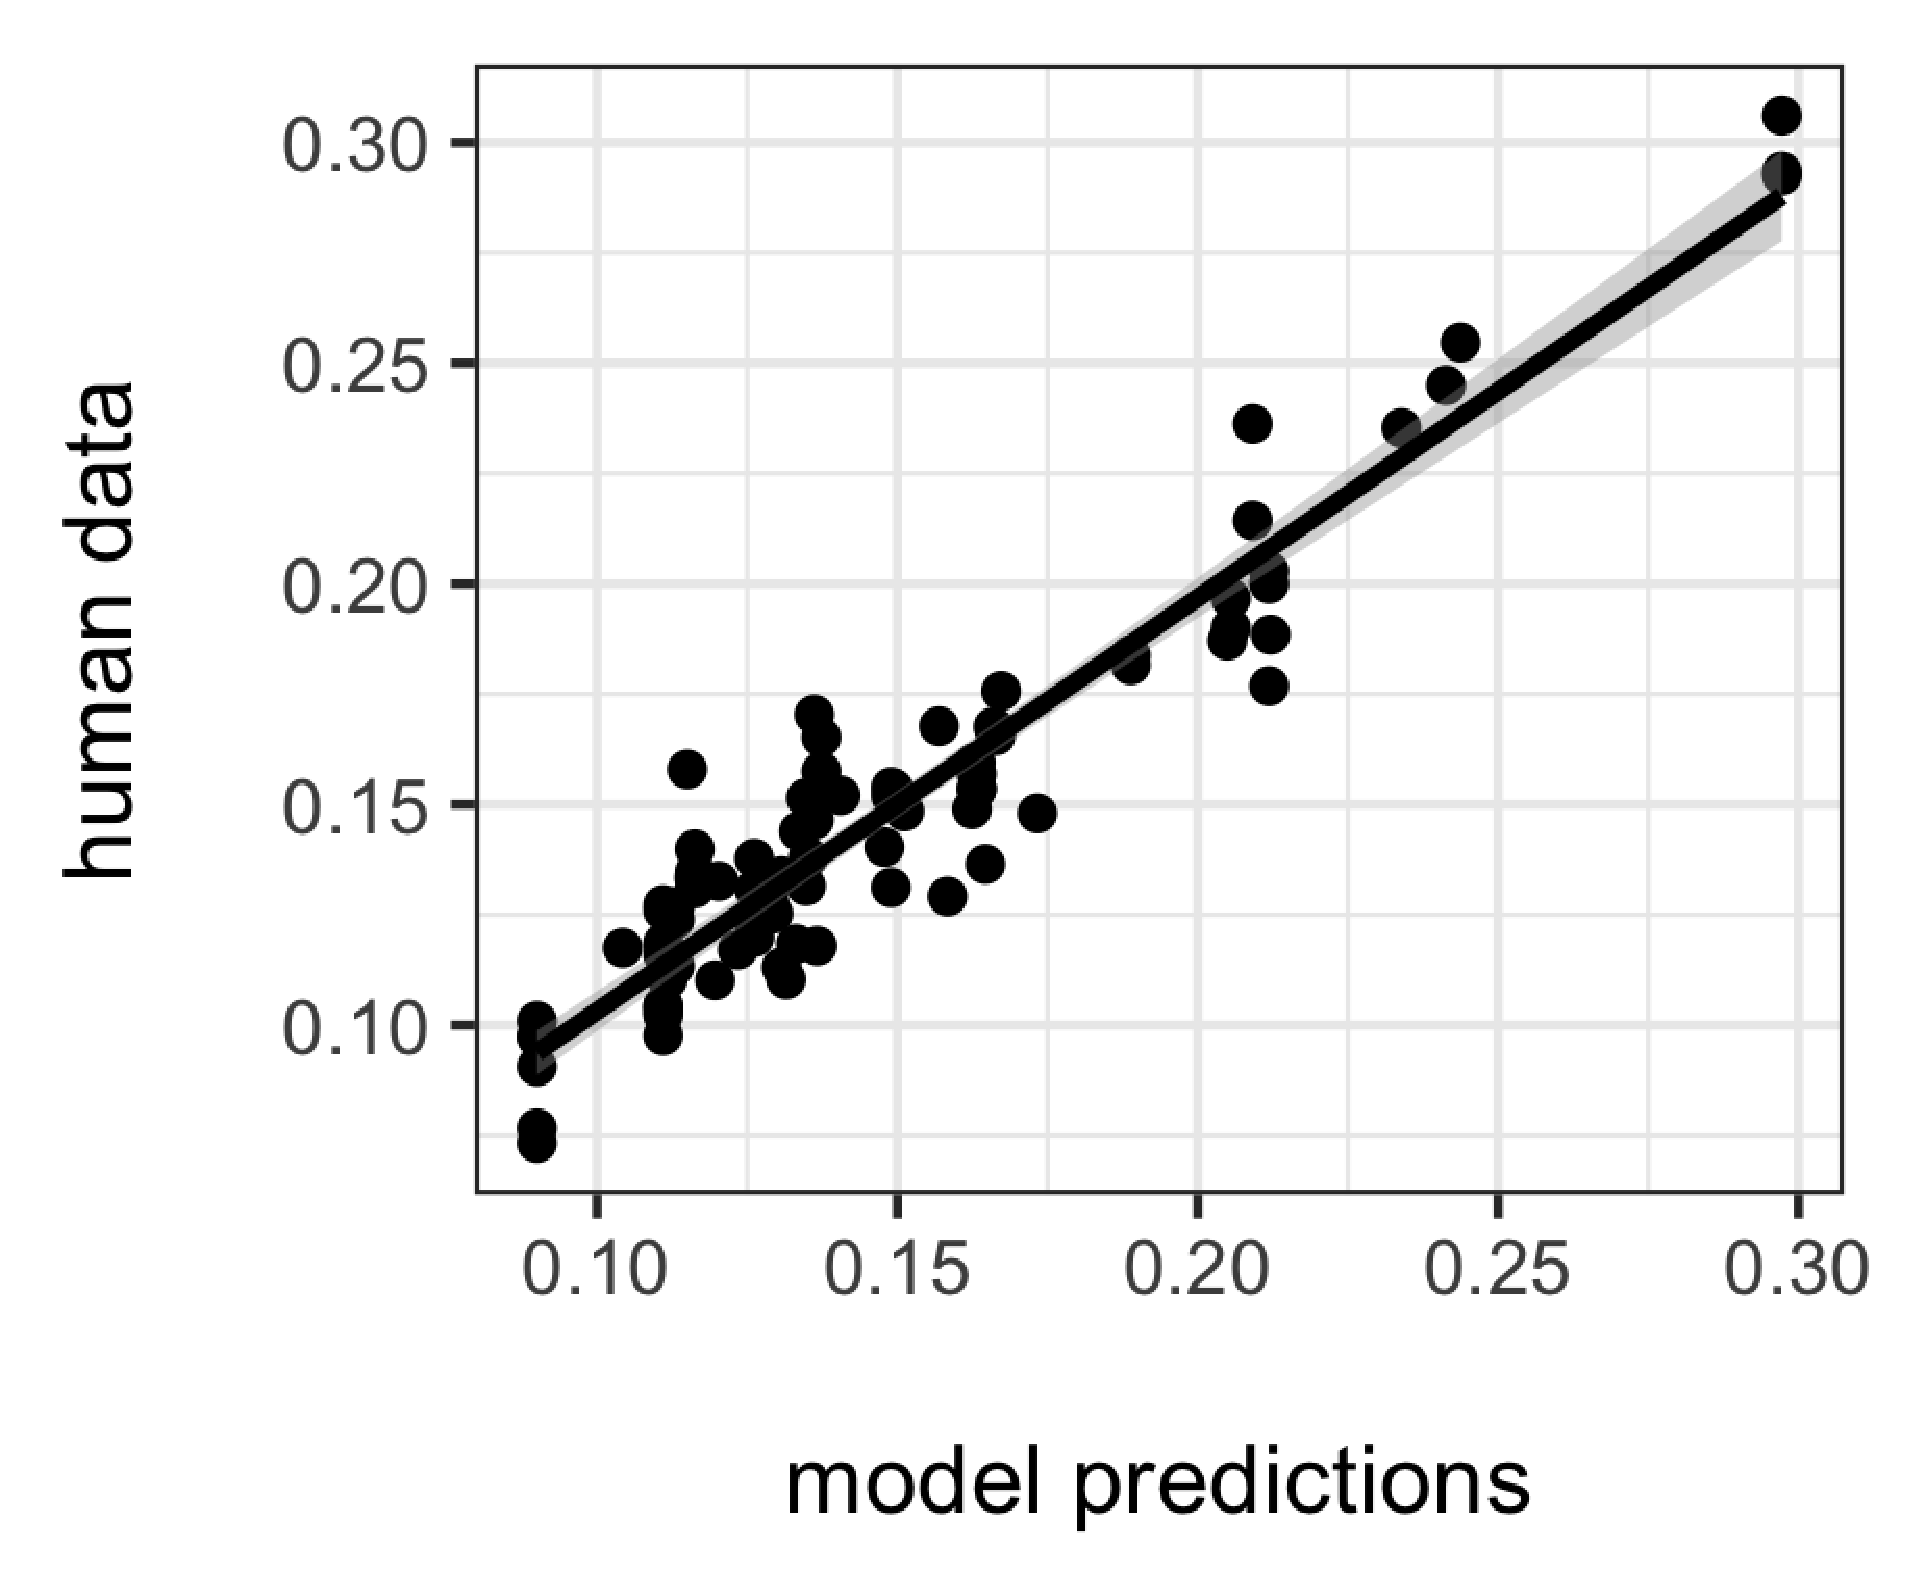
\includegraphics[width=3in]{images/X3-scatter-CogSci.eps}
	\caption{Experiment 2 results; $r^{2}=0.91$, 95\% CI [0.84, 0.85].}\label{exp2-results}
\end{figure}



% I recorded the same number of conditions as in Experiment 1. I think Experiment 2 used the same ambiguity code.

By reasoning about predictions of $S_2$, we are able to use our extended RSA model to compute the expected most informative utterance with respect to inferring preferences. In other words, $P_b(u)$ calculates the probability that a speaker would choose $u$ for the purpose of inferring preferences in our reference game scenario.
To generate predictions from $P_b(u)$, a total of three free parameters can be identified. 
As with the analysis for Experiment 1, we consider different values for $\alpha$ (i.e., speaker's soft may factor) and $\gamma$ (i.e., preference softness). 
We must also set the $\lambda$ parameter, which factors the importance of choosing expected most informative utterance with respect to the determined KL divergence values.
Note that when allowing negative values, negated information gain essentially minimizes expected information gain.
Thus, in this case the model would predict the choice of non-ambiguous utterances. 
Moreover, when $\lambda=0$ the model again collapses to a uniform distribution of utterance choices, thus yielding a nested model to a uniform base model. 


Again we optimized model values with respect to KL divergence estimates between the participant data and the model predictions---in this case for utterance preference distributions. 
The results for the uniform base model yielded an average KL divergence value of $5.415$ (median=$3.997$), while the model with $\lambda$ being optimized yields a mean KL divergence of $3.774$ (median=$2.108$).
Again determining $G^2$ to enable a Chi-square test for significant model differences in fitting the data, the difference between the base model and one parameter model (factored by $2*15=30$) of $49.23$ (median difference yields a value of $56.67$) is highly significant, indicating that the one-parameter model fits the data much better than a uniform base model. 
% Note: these interesting observations may not be mentioned _ I leave them in for now because the discussion can relate to them 
It is also interesting to report that three groups of participants could indeed be distinguished when considering the fitted parameter values of $\gamma$: 
a ``lazy worker'' group of $18$ participants yields values close to zero, i.e.,  $-.02 < \gamma<.02$.
The second group of $32$ participants yielded more negative values, i.e., $-8.20<\gamma<-.02$, indicating that a significant number of participants preferred to systematically choose non-ambiguous utterances. 
The third group of again $32$ participants yielded more positive values, i.e., $.02<\gamma<.47$, those choosing the most ambiguous utterance in a rather strategic manner. 


The proper model fit is confirmed when considering the correlation between the participants' data and the model.
As with Experiment 1, we averaged the data and the respective model predictions across specific case bins, which include all scenes that yield identical utterance choice options. 
In this case, $14$ distinct conditions can be identified, with a total of $84$ slider values to set. 
% Note: I did check it - there are indeed 14. 5+5+6+7+6+6+7+3+4+5+6+7+8+9
After matching the respective actual feature values with the utterance choice relevance within the respectively binned conditions, we again computed averages over utterance preference values for the respectively binned trials across participants and across respective model predictions. 


Figure \ref{exp2-results} plots predictions from the $\lambda$-optimized model, together with the human data. Again, we observe a positive correlation between the human judgments and model predictions ($r^2 = 0.91, p < 0.001$). In other words, we find evidence in support of the idea that speakers reason pragmatically about the relative informativity of ambiguous language.



\section{Discussion}

We have found strong support for our model of inferring priors on the basis of ambiguous language.
The results of Experiment 1 demonstrate that na\"ive speakers are able to reason pragmatically about \emph{why} listeners may take the actions they do, and the success of our computational model in predicting the observed behavior offers an articulated hypothesis about \emph{how} this reasoning proceeds: when speakers are aware of the ambiguity in their utterances, observing how listeners resolve that ambiguity provides clues to the preferences listeners use when doing so.
The results of Experiment 2 demonstrate that speakers are able to capitalize on this reasoning to strategically select utterances that are most likely to inform their understanding of the preferences of their listeners.
Crucially, the most informative utterances are also the most ambiguous ones.

Thus, this set of the experiments indicates that humans are very much aware of the fact that by observing responses, information about the listener's prior preferences can be inferred. 
Please note that ambiguous utterances are in this sense also related to questions, which may directly ask about preferences. 
However, it appears that in normal conversations, one often prefers to utter ambiguous statements, out of politeness reasons and possibly also because the conversation stays more natural and fluid.  
In this respect we also would like to emphasize that the analyzed preference prior, from a much more general perspective, can be interpreted as the general predictive state of mind of the listener while interpreting the utterance of the speaker \cite{Butz:2017}. 
Thus, this state of mind does not only include ``preferences'', but essentially all imaginable opinions, beliefs, and ibid. preferences of the listener. 
Moreover, during a conversation, this prior will obviously dynamically develop dependent on the internal predictive models and the generated utterances of speaker and listener, possibly characterizing it as the prior that depends on the current private grounds of the conversation partners and the common ground in which each of them assumes that the conversation unfolds. 


%Moreover, there 
%in conversation the priors dynamically unfold according to beliefs and preferences about the world and speakers
%twin anecdote, politeness (why not ask directly?)
%is ambiguity a feature that evolved under pressure from these considerations (i.e., informing preferences), or did ambiguity predate these considerations and speakers merely figured out clever ways of capitalizing on it---a lemonade-out-of-lemons scenario?

\bibliographystyle{apacite}
\setlength{\bibleftmargin}{.125in}
\setlength{\bibindent}{-\bibleftmargin}

\bibliography{prior-inference}

\end{document}

